\section{Actividad 6}

Armar Fig.~\ref{fig:3} en GNU Radio.  

\begin{figure}[H]
    \centering
    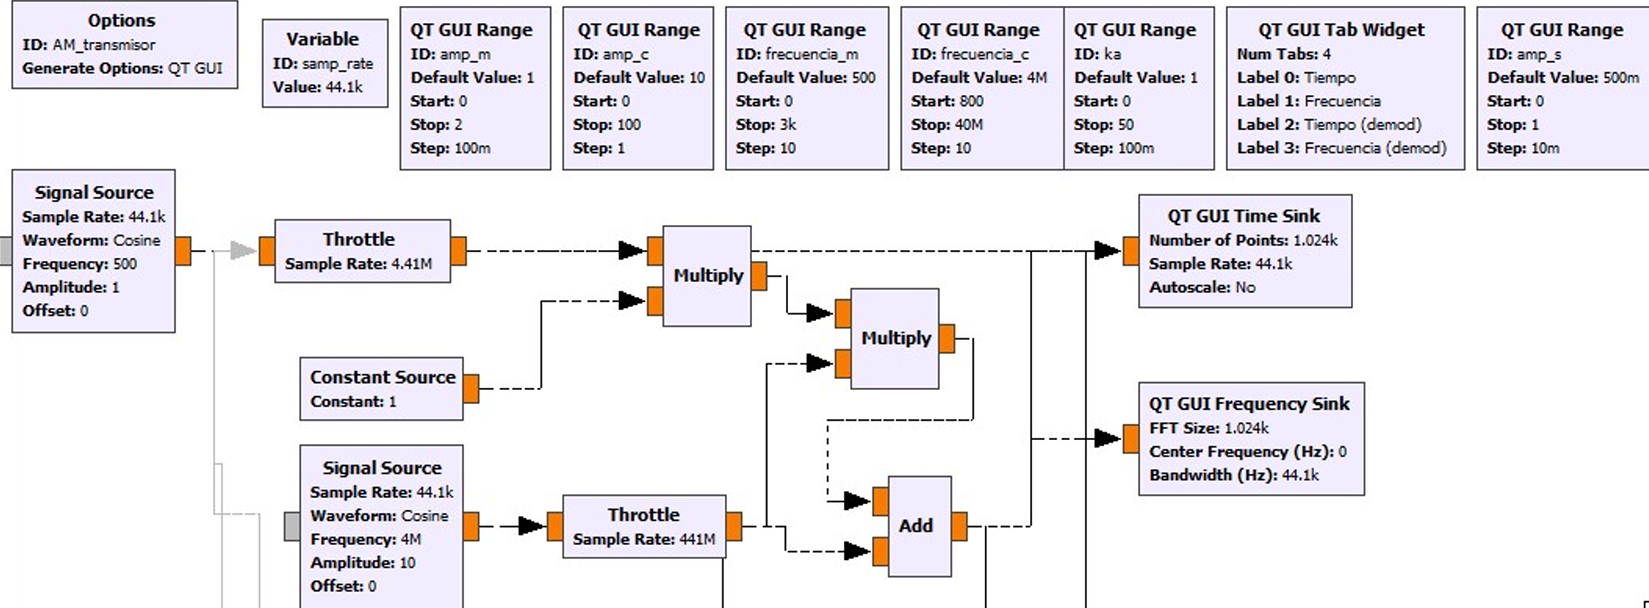
\includegraphics[width=0.9\textwidth]{imagenes/Parte_1/Actividad_6/fig3.png}
    \caption{Esquema en GNU Radio}
    \label{fig:3}
\end{figure}

\subsection*{a) ¿Qué es GNU Radio?}

GNU Radio es un entorno de desarrollo de software de código abierto y gratuito, el cual mediante bloques se puede realizar un procesamiento de señales para implementar radios de software. Se puede utilizar con hardware de RF externo de bajo costo o sin hardware en un entorno similar a una simulación.

\subsection*{b) ¿Qué es una SDR?}

SDR(Software Defined Radio) o radio definido por radio, está compuesta por una parte de hardware(radio frecuencia) y otra parte basada en Software. Estas se caracterizan en poder programar el tráfico y control de la información, soportando un amplio rango de frecuencias y aplicaciones de software.
Además de modificar y obtener un formato de comunicación a otro en cuestión de milisegundos.

\subsection*{c) Expresar matemáticamente la señal modulada $s(t)$ del modulador AM del esquema.}

Analizando el esquema de la Figura \ref{fig:3}, se obtiene que la se~nal modulada $s(t)$ posee la siguiente expresión:

    $$s(t) = A_c [1 + K_aA_m]cos(2\pi f_c t)$$

\subsection*{d) Explicar brevemente qué realizan cada uno de los bloques de la Fig.~3.}

\begin{itemize}
    \item \textbf{Signal source:} Permite generar distintas señales de onda, cosenoidales, senoidales, constantes, triangulares y diente de sierra, permitiendo modificar los parámetros de amplitud, frecuencia, seleccionar un offset y el tipo de variable que se desee en la salida del bloque, es decir si es compleja, entera, etc.
    \item \textbf{Multiply:} Realiza la multiplicación de señales.
    \item \textbf{Add:} Realiza la adición o suma de señales.
    \item \textbf{Trhottle:} Es un acelerador de muestras, de esta forma, la tasa promedio no excede la tasa específica, hablando en muestras por segundo.
    \item \textbf{QT GUI Range:} es un elemento de control gráfico que permite crear un deslizador (slider) en la interfaz QT de GNU Radio Companion. Su función principal es proveer un valor variable (por ejemplo, frecuencia, ganancia, amplitud, etc.) que el usuario puede ajustar en tiempo real durante la ejecución del diagrama de flujo.
    \item \textbf{Constant Source:} es un bloque de fuente de datos, es decir, genera una señal constante en el tiempo (una secuencia de muestras con un valor fijo), que puede usarse para alimentar otros bloques del sistema.
    \item \textbf{QT GUI Tab Widget:} es un bloque gráfico de interfaz que permite organizar múltiples visualizaciones o controles en pestañas (tabs) dentro de la ventana QT. No procesa señales, pero es muy útil para estructurar y ordenar la interfaz gráfica cuando tenés varios elementos (como sliders, gráficas FFT, osciloscopios, etc.).
    \item \textbf{Variable:} es uno de los elementos más fundamentales, no procesa señales ni genera gráficos, sino que define un valor que puede ser usado en todo el diagrama de flujo como si fuera una constante simbólica o un parámetro global.
    \item \textbf{Options:} es especial porque no representa ni un bloque de procesamiento ni un control gráfico, sino que define las configuraciones globales del diagrama de flujo. En otras palabras, es el “bloque principal” que le dice a GNU Radio cómo debe ejecutarse el resto del sistema.
    \item \textbf{QT GUI Time Sink:} es uno de los bloques más usados para visualizar señales en el dominio del tiempo en tiempo real. Funciona como un osciloscopio digital, mostrando la evolución temporal de una o varias señales que recibe como entrada.
    \item \textbf{QT GUI Frequency Sink:} es el equivalente a un analizador de espectro en tiempo real. Su función es mostrar la distribución espectral de una o varias señales, es decir, cómo se reparte la energía de la señal en función de la frecuencia.
\end{itemize}

\subsection*{e) Obtener las gráficas para un porcentaje de modulación del 10\%, 60\% y 100\%.}

\begin{figure}[H]
    \centering
    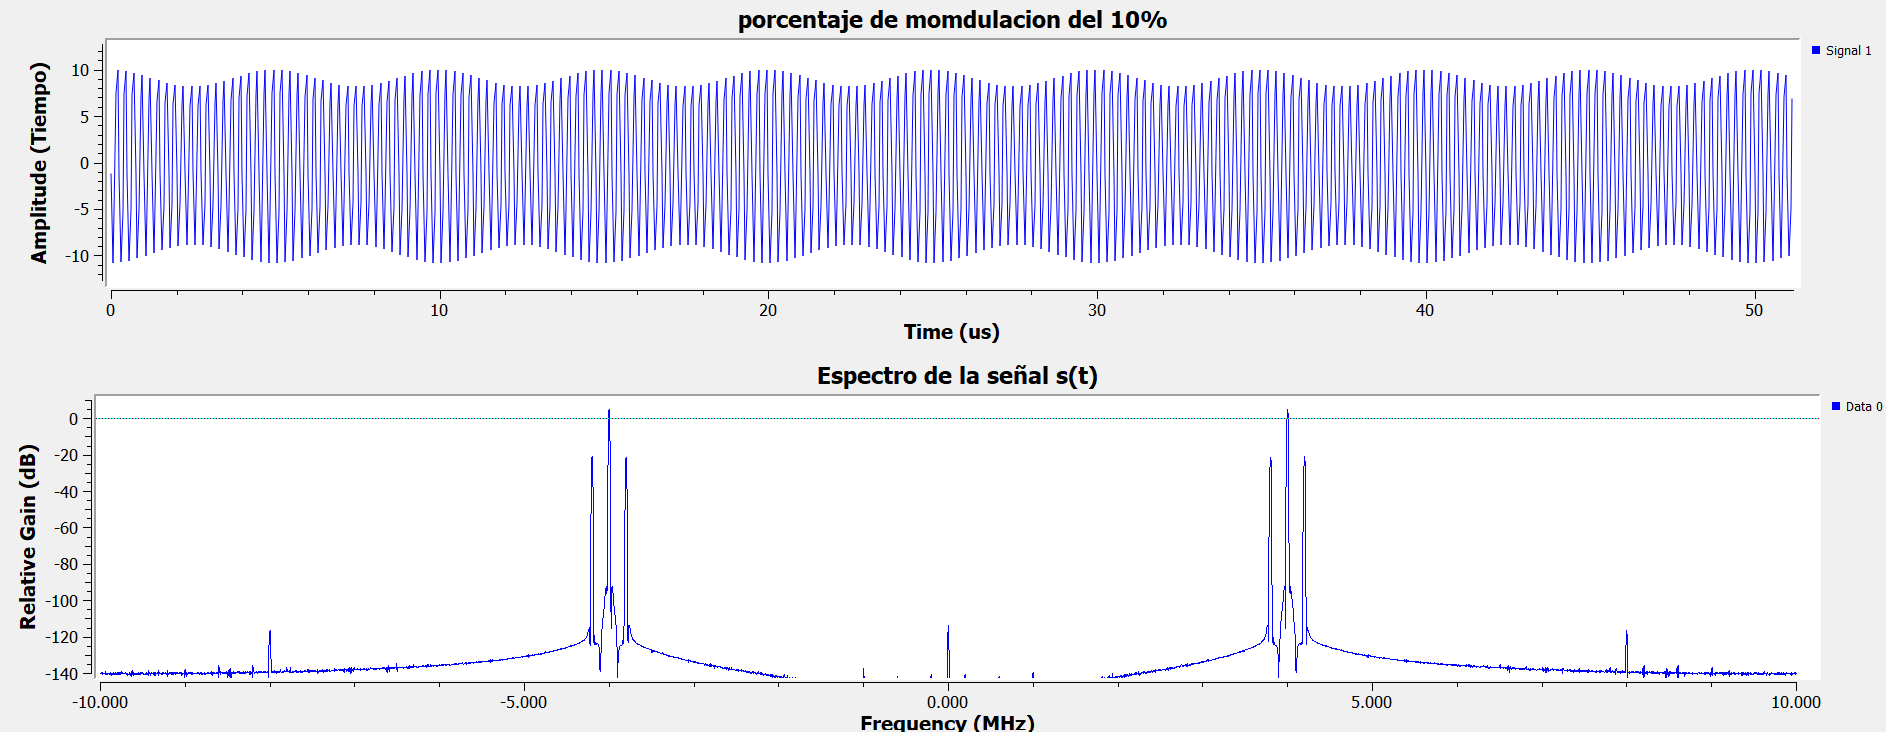
\includegraphics[width=0.9\textwidth]{imagenes/Parte_1/Actividad_6/modulacion_al_10.png}
    \caption{Modulación al 10\%}
    \label{fig:8}
\end{figure}

\begin{figure}[H]
    \centering
    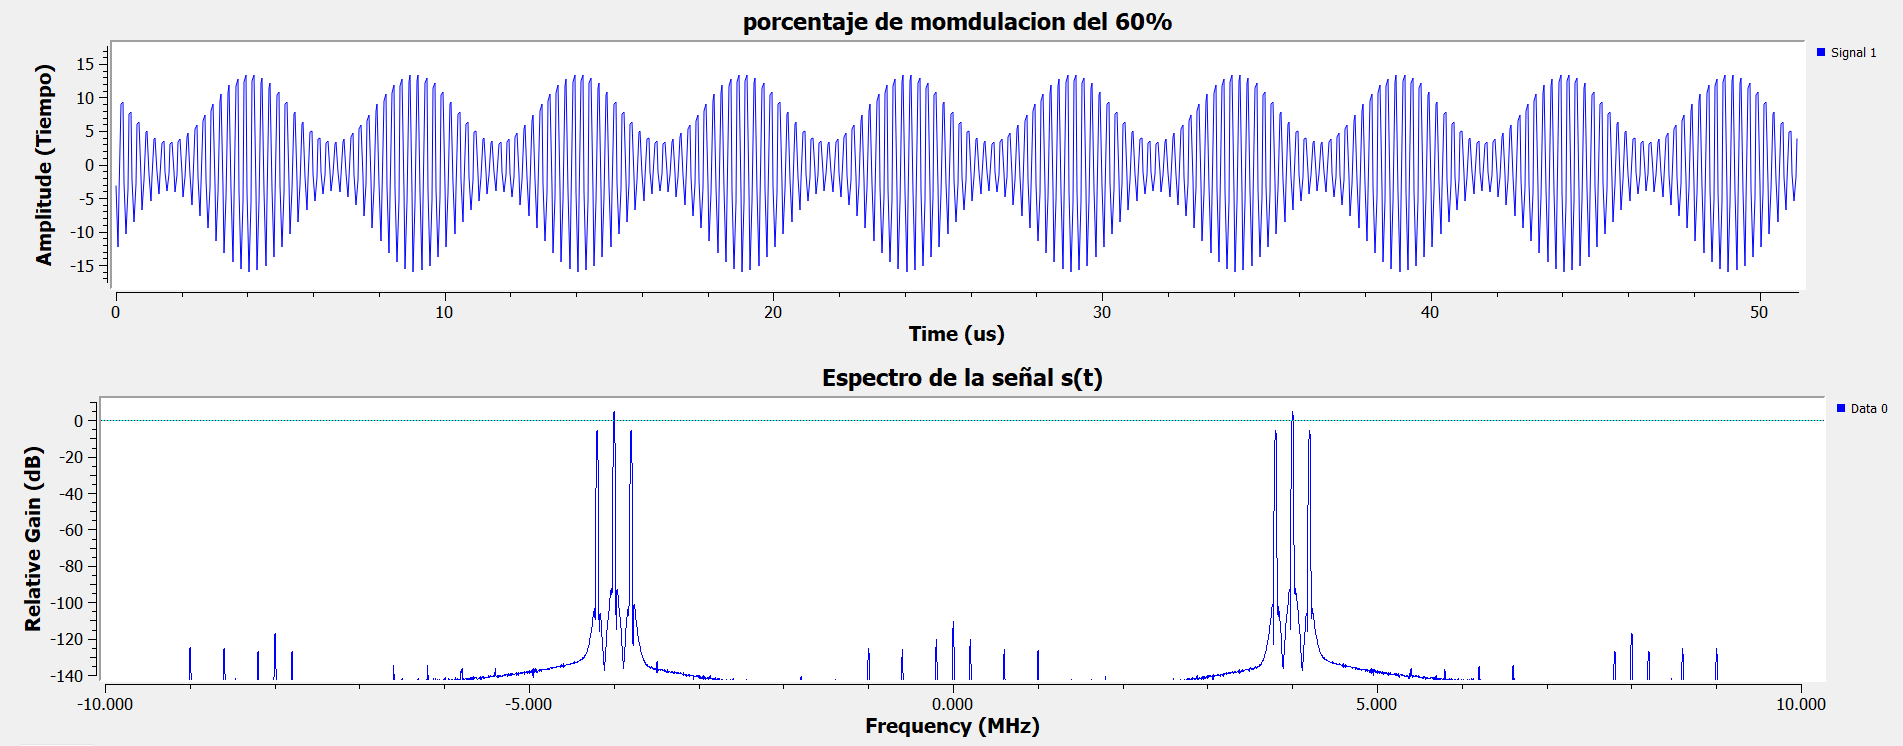
\includegraphics[width=0.9\textwidth]{imagenes/Parte_1/Actividad_6/modulacion_al_60.png}
    \caption{Modulación al 60\%}
    \label{fig:9}
\end{figure}

\begin{figure}[H]
    \centering
    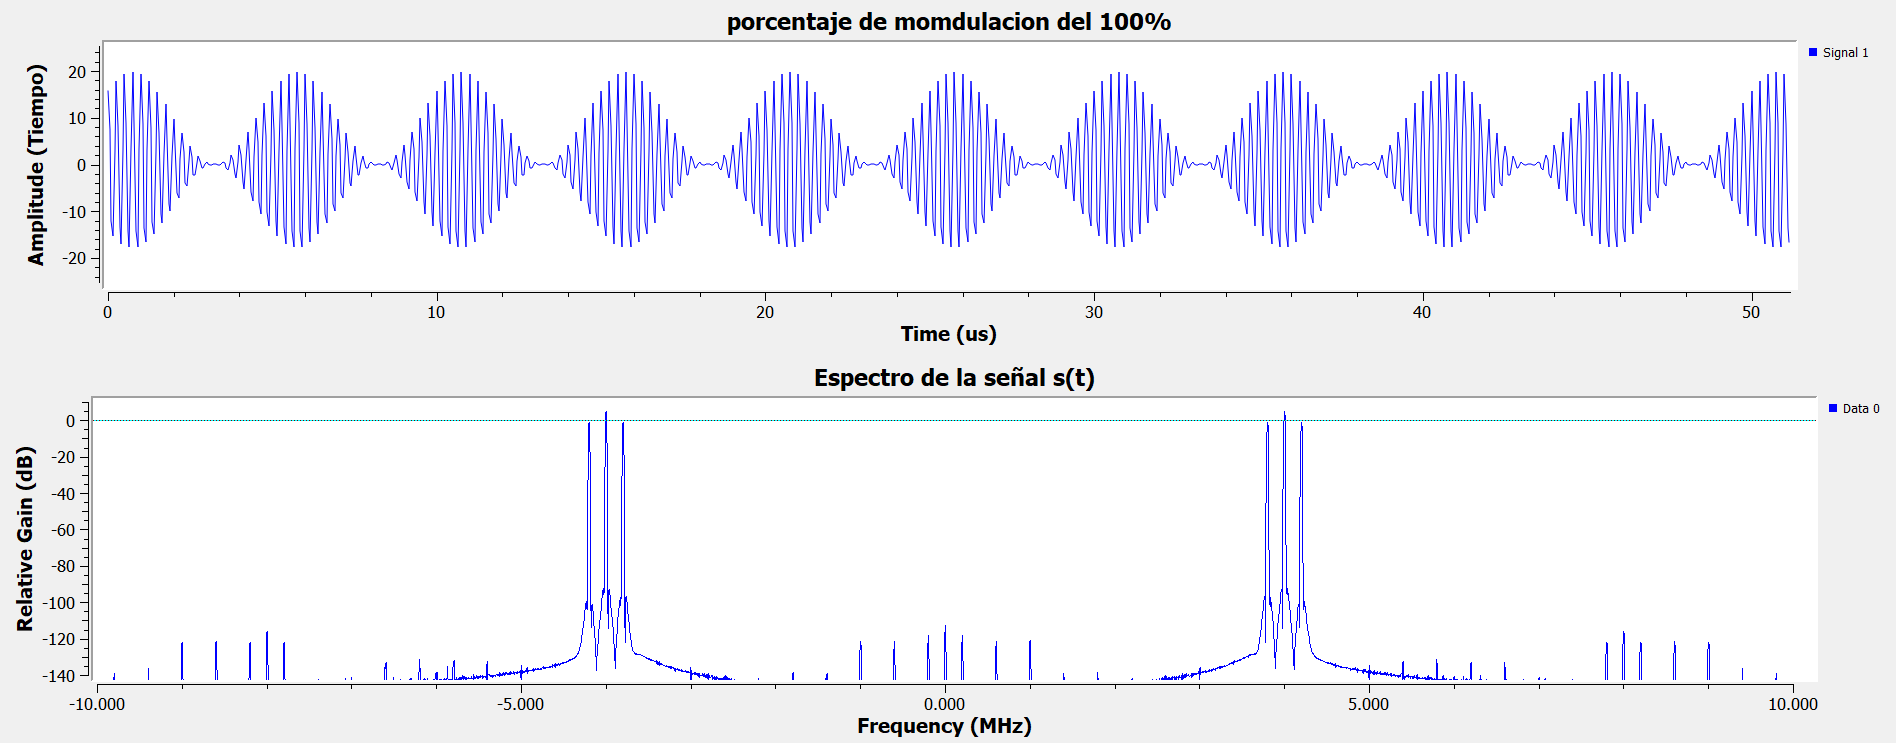
\includegraphics[width=0.9\textwidth]{imagenes/Parte_1/Actividad_6/modulacion_al_100.png}
    \caption{Modulación al 100\%}
    \label{fig:10}
\end{figure}


\subsection*{f) Obtener la gráfica con sobre-modulación en la señal $s(t)$.}

\begin{figure}[H]
    \centering
    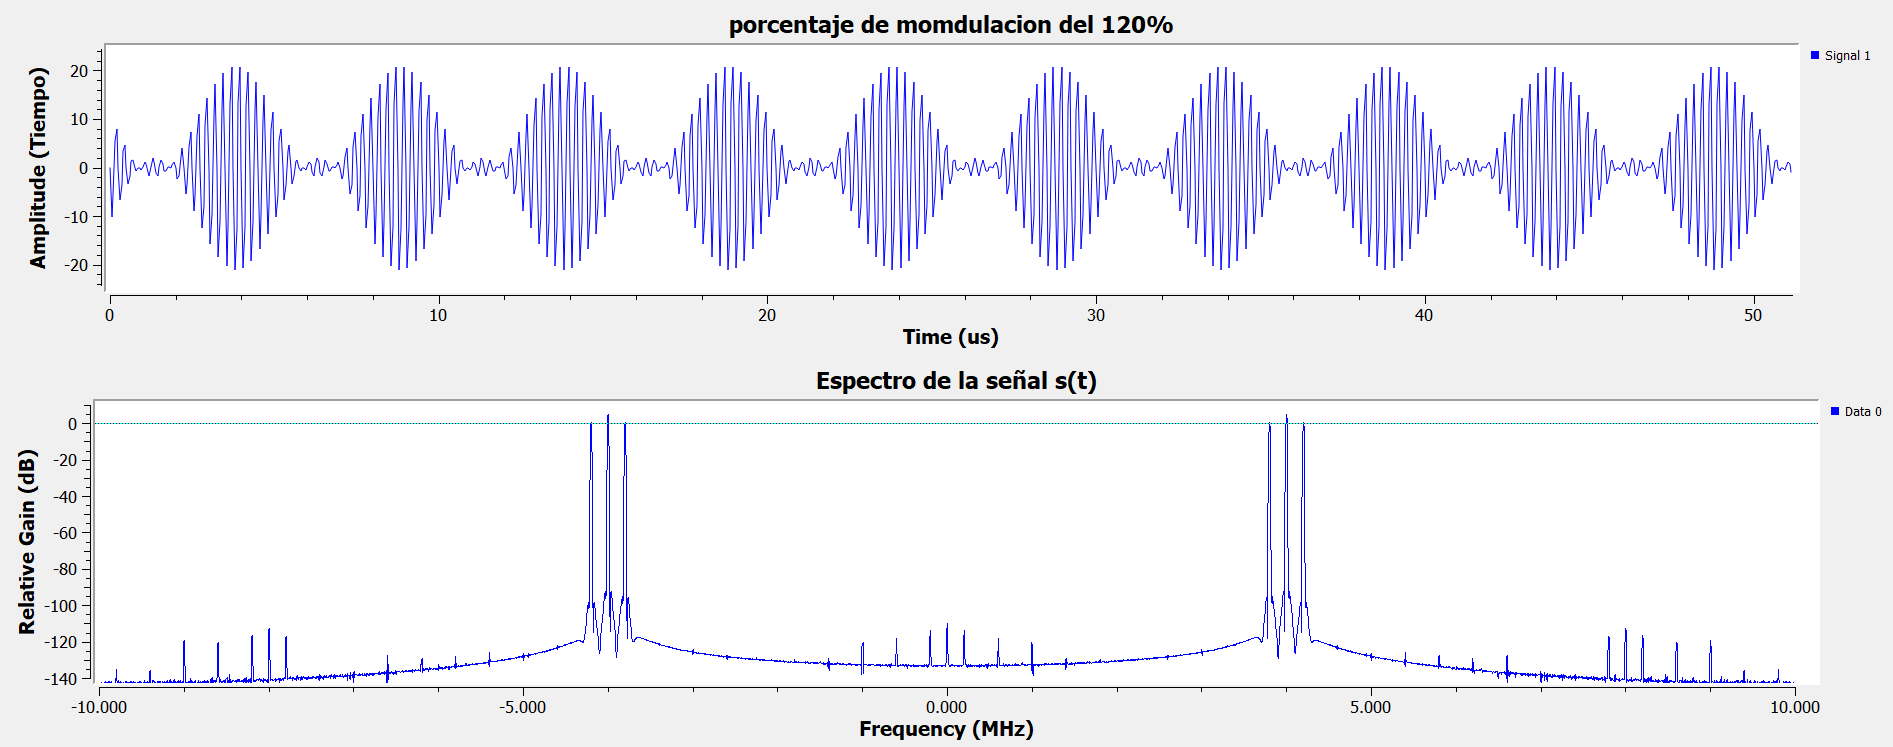
\includegraphics[width=0.9\textwidth]{imagenes/Parte_1/Actividad_6/sobremodulacion.png}
    \caption{Sobre-modulación}
    \label{fig:11}
\end{figure}

\subsection*{g) Analizar qué sucede con el espectro de la señal en cada uno de los casos planteados en d) y e). Indicar en el informe las gráficas obtenidas.}

En las Fig. \ref{fig:8}, \ref{fig:9}, \ref{fig:10} y \ref{fig:11} se puede apreciar el espectro de la señal para el porcentaje de modulación correspondiente, al observar estos espectros se logra apreciar que a medida que el porcentaje de modulación va aumentando, la amplitud de las bandas lateras también aumenta mientras la amplitud de la portadora permanece constante.

\subsection*{h)Implementar un receptor y obtener la señal original.}

En la Fig.\ref{fig:ejercicio_6h} se muestra el espectro de la señal demodulada.

    \begin{figure}[H]
        \centering
        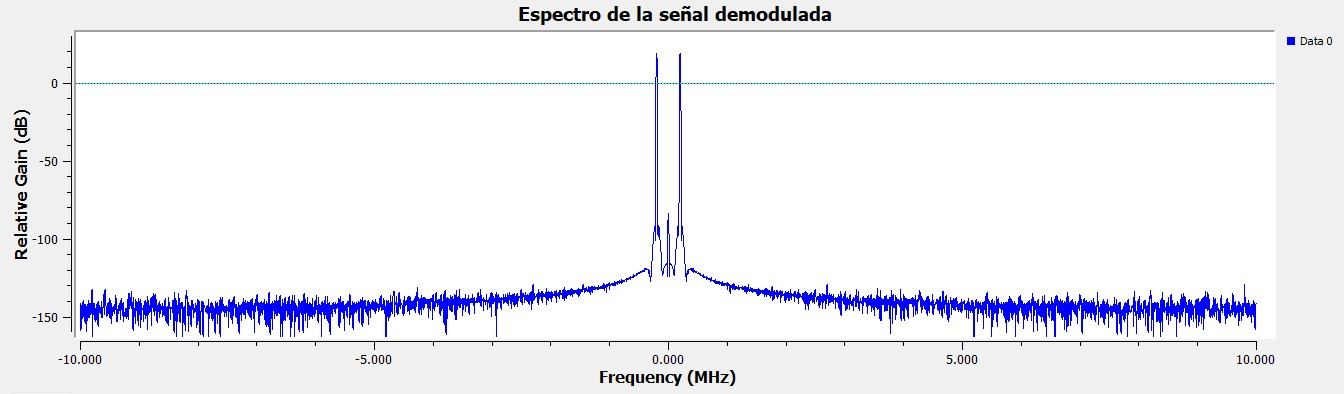
\includegraphics[width=0.9\linewidth]{imagenes/Parte_1/Actividad_6/ejercicio_6h.jpg}
        \caption{Señal demodulada.}
        \label{fig:ejercicio_6h}
    \end{figure}